\documentclass[../main.tex]{subfiles}
\begin{document}

\section{Potential Fields for Obstacle Avoidance  \\ \normalfont\normalsize\texttt{Emil Vincent Ancker}}
\label{sec:avoidance}
In this section simple spherical obstacles will be considered. The problem under consideration are obstacles being located on the trajectory of the end-effector, which is visualized in \autoref{fig:DMP:obstacle}.

\begin{figure}[H]
    \centering
         \includegraphics[width=0.50\textwidth]{figures/DMP/obstacle.png}
     \caption{Trajectory demonstration and fitted DMP with introduction of a spherical obstacle.}
     \label{fig:DMP:obstacle}
\end{figure}

To avoid collision with the obstacle, the obstacle will need to be incorporated into the trajectory generation.

As stated previously obstacle avoidance can be incorporated into the DMP framework by adding a new term in the transformation system presented in \autoref{eq:system:transformation}. A potential field, $C_t$, which repels the manipulator away from obstacles is added to the transformation system.
\begin{align} \label{eq:system:transformation}
    \tau \dot{\boldsymbol{z}} &= \alpha_z  (\beta_z ( \boldsymbol{g} - \boldsymbol{x} ) - \boldsymbol{z} ) + f + C_t,\\
    \nonumber \tau \dot{\boldsymbol{x}} &= \boldsymbol{z}, 
\end{align}
There are many ways to define the potential field, some of these will be implemented and evaluated in this section.

\subsection{Potential Field as a Function of Steering Angle \\ \normalfont\normalsize\texttt{Emil Vincent Ancker}}

In the work \cite{warren_behavioral_2010} a simple function for human obstacle avoidance is presented:
\begin{equation} \label{eq:human:avoidance}
    \dot{\theta} = \gamma_0 \theta e^{-\beta_0|\theta|}
\end{equation}
Where $\gamma_0$ and $\beta_0$ are constants and $\theta$ is the angle between the velocity of the end effector and the vector extended from the end effector to the obstacle.

\begin{figure}[H]
\begin{center}
        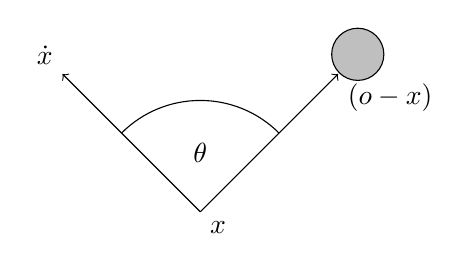
\begin{tikzpicture}
        % Defining nodes
        \node[below right] (R) at (0,0) {$\boldsymbol{x}$};
        \node[draw, shape=circle,fill=lightgray, xscale = 2.0, yscale=2.0] (R1) at (2, 2) {};
        \node[below right] (ox) at (1.75,1.75) {$(\boldsymbol{o}-\boldsymbol{x})$};
        \draw[->] (0,0)--(1.75, 1.75);
        \draw[->] (0,0)--(-1.75,1.75);
        \node[above left] (v) at (-1.75,1.75) {$\dot{\boldsymbol{x}}$};
        \draw (1,1) arc[radius=1.4142,start angle=45,end angle=135];
        \node[] (R) at (0,0.75) {$\theta$};
    \end{tikzpicture}
\end{center}
\caption{Illustration of steering angle $\theta$, where $\boldsymbol{x}$ is the end-effector position, $\dot{\boldsymbol{x}}$ is the end-effector velocity and the vector $(o-x)$ is the vector from the end-effector to the obstacle.}
\label{fig:dmp:steering_angle}
\end{figure}

In \cite{rai_learning_2014} a potential field based on \autoref{eq:human:avoidance} is presented:
\begin{equation}
    C_t = \gamma_0 R \dot{\boldsymbol{x}} \theta e^{-\beta_0 |\theta|}
\end{equation}
The steering angle in \autoref{fig:dmp:steering_angle} can simply be calculated by finding the angle between the vectors $\boldsymbol{(o-x)}$ and $\boldsymbol{\dot{x}æ}$ on the plane where the vectors lie. 
\begin{align}
    \theta = \text{cos}^{-1}\left(\frac{\boldsymbol{(o-x)}^T\dot{\boldsymbol{x}}}{|\boldsymbol{(o-x)}| |\dot{\boldsymbol{x}}|}\right)
\end{align}
The rotation $R$ is simply a rotation of $\frac{\pi}{2}$ around the normal of the plane where $\boldsymbol{(o-x)}$ and $\dot{\boldsymbol{x}}$ lies:
\begin{equation}
    \boldsymbol{n} = \boldsymbol{(o-x)} \times \dot{\boldsymbol{x}}
\end{equation}
The rotation matrix $R$ can be found from transforming an angle axis rotation of angle $\frac{\pi}{2}$ around the vector $\boldsymbol{n}$:
\begin{equation}
    R = [\boldsymbol{n}]_{\times} + \boldsymbol{n}\boldsymbol{n}^T
\end{equation}
Where $[\boldsymbol{n}]_{\times}$ is the skew symmetric matrix of $\boldsymbol{n}$.

\subsubsection{Evaluation of Steering Angle Based DMP \\ \normalfont\normalsize\texttt{Emil Vincent Ancker}} \label{subsubsec:eval:steering:dmp}
When adjusting the tuning parameters of the potential field ($\gamma$, $\beta$), there are multiple external factors which also have an effect. The end-effector velocity $\dot{\boldsymbol{x}}$ has a direct effect on the choice of $\gamma$, since following a trajectory with higher velocity would lead to a repulsive force of higher magnitude shown in \autoref{eq:human:avoidance}.
\begin{equation}
    \uparrow \dot{\boldsymbol{x}} \quad \Rightarrow \quad \downarrow \gamma_0
\end{equation}
Furthermore, the shape of the obstacle has an influence on the tuning of the parameters. The parameter $\beta$ determine the sensitivity of the steering angle:
\begin{align}
    \uparrow \beta_0 \quad &\Rightarrow \quad \text{lower sensitivity span of steering angle} \\
    \downarrow \beta_0 \quad &\Rightarrow \quad \text{higher sensitivity span of steering angle}
\end{align}
In other words, if $\beta$ is chosen high, the DMP only avoids the obstacle if it is almost directly in front of it. But if $\beta$ is chosen too low it might incorporate obstacles in the motion that are too far to the side.

\begin{figure}[H]
    \centering
    \begin{subfigure}[b]{0.48\textwidth}
        \centering
        \includegraphics[width=\textwidth]{figures/DMP/obstacle_simple_dmp.png}
        \caption{Trajectories visualized in cartesian space.}
        \label{fig:dmp:obstacle:simple:1}
    \end{subfigure}
    \hfill
    \begin{subfigure}[b]{0.48\textwidth}
        \centering
        \includegraphics[width=\textwidth]{figures/DMP/obstacle_simple_dmp_2.png}
        \caption{Trajectory shown in X, Y and Z axes.}
        \label{fig:dmp:obstacle:simple:2}
    \end{subfigure}
    \caption{Results for using a potential fields which only takes steering angles into account with the following tuning variable values: $\gamma_0 = 10^6$, $\beta_0 = \frac{20}{\pi}$. Obstacle is a sphere with $r=0.025[m]$ located at  $xyz=[0.0, 0.25, 0.80]$.}
    \label{fig:dmp:obstacle:simple}
\end{figure}

An example of parameters that is well adjust to the demonstration is shown in \autoref{fig:dmp:obstacle:simple}. But there are numerous problems with this potential field, which can be seen from \autoref{eq:human:avoidance}. If the end-effector is heading directly towards the obstacle, $\theta = 0$, then it will not get repelled by the potential field since the magnitude is zero. Furthermore, obstacles far away have an influence on the motion, which is shown in \autoref{fig:dmp:obstacle:problem}. 

\begin{figure}[H]
    \centering
    \begin{subfigure}[b]{0.48\textwidth}
        \centering
        \includegraphics[width=\textwidth]{figures/DMP/obstacle_problem_1.png}
        \caption{Trajectories visualized in cartesian space.}
        \label{fig:dmp:obstacle:problem:1}
    \end{subfigure}
    \hfill
    \begin{subfigure}[b]{0.48\textwidth}
        \centering
        \includegraphics[width=\textwidth]{figures/DMP/obstacle_problem_2.png}
        \caption{Trajectory shown in X, Y and Z axes.}
        \label{fig:dmp:obstacle:problem:2}
    \end{subfigure}
    \caption{Problem of obstacles far away visualized with the following tuning variable values: $\gamma_0 = 10^6$, $\beta_0 = \frac{20}{\pi}$. Obstacle is a sphere with $r=0.025[m]$ located at  $xyz=[0.0, 0.25, 0.80]$.}
    \label{fig:dmp:obstacle:problem}
\end{figure}

\subsection{Potential Fields with Coupled Terms \\ \normalfont\normalsize\texttt{Mikkel Larsen}}
In order to counteract the problems stated above where when the angle $\theta=0$ the repelling force yielded $C_t=0$ and the potential field always has an impact on the motion no matter the distance, the paper \cite{rai_learning_2014} presented a new potential field which is shown in \autoref{eq:pot:coupled:terms}. 

\begin{equation} \label{eq:pot:coupled:terms}
     C_t = \gamma_1 R \dot{\boldsymbol{x}}\phi_1 +  \gamma_2 R \dot{\boldsymbol{x}}\phi_2 +  \gamma_3 R \dot{\boldsymbol{x}}\phi_3
\end{equation}

Furthermore the new potential field does also consider nearest point on the obstacle seen from the end-effector instead of just using the center of the obstacle. This is particularly important when dealing with non-uniform obstacles, because only using the center of the obstacle could lead to collision. The three coupling terms $\phi_1, \phi_2, \phi_3$ are defined as
\begin{align}
    \phi_1 = \theta e^{-\beta_0 |\theta|} \cdot e^{-kd} \\
    \phi_2 = \theta e^{-\beta_0 |\theta_p|} \cdot e^{-kd_p} \\
    \phi_3 =  e^{-kd} 
\end{align}

Where $k$ is a constant, $d$ is the distance to the center of the object from the end-effector, $\theta_p$ is the angle from the end-effector to the nearest point on the object and $d_p$ is the distance from the end-effector to the nearest point on the object. From the coupling terms it can be seen the term $e^{-kd}$ scales the potential field with the distance, where the longer away from the obstacle the less effect from the repulsive force. This results in $\phi_1$ and $\phi_2$ are repulsive forces away from the obstacle center and nearest point on the object respectively taking the angle $\theta$ into account, and $\phi_3$ is a repulsive force which is used when the angle $\theta=0$.

\subsubsection{Evaluation of Potential Fields with Coupled Terms DMP \\  \normalfont\normalsize\texttt{Mikkel Larsen}} \label{subsubsec:eval:pot:coupled:term}

The following parameters ($\gamma_1, \gamma_2, \gamma_3$, $k$) of the potential field with coupled terms needs to be adjusted, where $\dot{\boldsymbol{x}}$ still has the same effect on $\gamma_i$ as described in \autoref{subsubsec:eval:steering:dmp}. The parameter $k$ scales the distance to the object meaning:
\begin{align}
    \uparrow k \quad &\Rightarrow \quad \text{Lesser impact of the distance to the object} \\
    \downarrow k \quad &\Rightarrow \quad \text{Higher impact of the distance to the object}
\end{align}
This means if $k$ is chosen to be high, the DMP can get closer to the object before the repulsive field has an impact and the opposite effect if $k$ is chosen to be low. With $\beta_0 = \frac{20}{\pi}$ and $k=15$ the repulsive field from $\phi_1$ and $\phi_3$ is activated around a distance of $d=0.3$ which was deemed acceptable. This is illustrated in \autoref{fig:coup:term:k}.   

\begin{figure}[H]
    \centering
    \begin{subfigure}[b]{0.48\textwidth}
        \centering
        \includegraphics[width=\textwidth]{figures/DMP/dmp_coupled_terms_phi3.png}
        \caption{Coupling term $\phi_3$ versus distance to object center $d$.}
    \end{subfigure}
    \hfill
    \begin{subfigure}[b]{0.48\textwidth}
        \centering
        \includegraphics[width=\textwidth]{figures/DMP/dmp_coupled_terms_phi1.png}
        \caption{Coupling term $\phi_1$ versus distance to object center $d$ and angle to object center $\theta$}
    \end{subfigure}
    \caption{Plot of coupling term $\phi_3$ and $\phi_1$ with $k=15$ and $\beta_0 = \frac{20}{\pi}$.}
    \label{fig:coup:term:k}
\end{figure}

Next the same performance evaluation is done for DMP with potential fields with coupled terms as done for DMP with steering angle to compare them to each other. However, because the test is done with a sphere as an object, the nearest point on the obstacle does not have an impact and therefore $\gamma_2=0$. \autoref{fig:dmp:coup:obstacle:on:path} shows the performance for an sphere with radius $r=0.025[m]$ located on the trajectory at $xyz=[0.575, 0.30, 0.45]$ . 

\begin{figure}[H]
    \centering
    \begin{subfigure}[b]{0.48\textwidth}
        \centering
        \includegraphics[width=\textwidth]{figures/DMP/simple_traj_w_couple_terms_cartesian.png}
        \caption{Trajectories visualized in cartesian space.}
        \label{fig:dmp:coup:obstacle:on:path:1}
    \end{subfigure}
    \hfill
    \begin{subfigure}[b]{0.48\textwidth}
        \centering
        \includegraphics[width=\textwidth]{figures/DMP/simple_traj_w_couple_terms_xyz.png}
        \caption{Trajectory shown in X, Y and Z axes.}
        \label{fig:dmp:coup:obstacle:on:path:2}
    \end{subfigure}
    \caption{Results for using a potential field with coupling terms with the following tuning variable values: $\gamma_1 = 10^6$,  $\gamma_2=0$, $\gamma_3=1.25\cdot10^4$, $\beta_0 = \frac{20}{\pi}$, $k=15$. Obstacle is a sphere with $r=0.025[m]$ located at  $xyz=[0.575, 0.30, 0.45]$.}
    \label{fig:dmp:coup:obstacle:on:path}
\end{figure}

Looking at the trajectory using coupling terms at \autoref{fig:dmp:coup:obstacle:on:path:1} compared to the trajectory using only steering angle at \autoref{fig:dmp:obstacle:simple:1} it is seen the obstacle avoidance is nearly the same. However, after the obstacle has been avoided, the trajectory using coupling terms is corrected more onto the demonstrated path compared to the DMP trajectory only using steering angle. This is the result of taking the distance to the object into consideration. To further illustrate that the DMP trajectory using coupling terms follows the demonstrated path more than DMP trajectory only using steering angle the euclidean distance between the demonstrated path and the DMP generate path is calculated for both the coupling term DMP and the steering angle DMP. This is illustrated in \autoref{fig:angle:vs:coupled} where the same sphere parameters and DMP parameters are used as in \autoref{fig:dmp:coup:obstacle:on:path} and \autoref{fig:dmp:obstacle:simple} for coupling term DMP and steering angle DMP respectively. 

\begin{figure}[H]
    \centering
         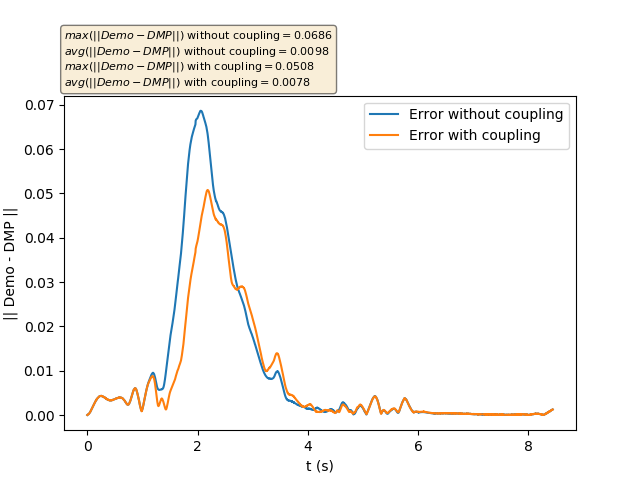
\includegraphics[width=0.6\textwidth]{figures/eval_trajectories/angle_based_v_couple_term.png}
     \caption{Euclidean distance between the demonstrated path and the DMP generated paths for DMP with coupling terms and DMP with steering angle. Path for DMP with coupling terms is the same as in \autoref{fig:dmp:coup:obstacle:on:path} and path for DMP with steering is the same as in \autoref{fig:dmp:obstacle:simple}.}
     \label{fig:angle:vs:coupled}
\end{figure}

\autoref{fig:angle:vs:coupled} confirms that the DMP with coupling terms follows the demonstrated path more accurate than the DMP with steering angle. Furthermore, it is seen that the obstacle is avoided around the $2$ seconds mark because of the high spike in difference between demonstrated path and DMP path. The DMP with coupling terms has $25.9 \%$ smaller maximum euclidean distance and $25.6 \%$ smaller average euclidean distance compared to DMP with steering angle.


The performance when an obstacle is away from the trajectory is illustrated in \autoref{fig:dmp:coup:obstacle:away:path}. Compared to DMP only using steering angle shown in \autoref{fig:dmp:obstacle:problem} the DMP trajectory is untouched. Again this is the result of taking the distance to the object into consideration. 

\begin{figure}[H]
    \centering
    \begin{subfigure}[b]{0.48\textwidth}
        \centering
        \includegraphics[width=\textwidth]{figures/DMP/obs_away_traj_w_couple_terms_cartesian.png}
        \caption{Trajectories visualized in cartesian space.}
        \label{fig:dmp:coup:obstacle:away:path:1}
    \end{subfigure}
    \hfill
    \begin{subfigure}[b]{0.48\textwidth}
        \centering
        \includegraphics[width=\textwidth]{figures/DMP/obs_away_traj_w_couple_terms_xyz.png}
        \caption{Trajectory shown in X, Y and Z axes.}
        \label{fig:dmp:coup:obstacle:away:path:2}
    \end{subfigure}
    \caption{Results for using a potential field with coupling terms with the following tuning variable values: $\gamma_1 = 10^6$,  $\gamma_2=0$, $\gamma_3=1.25\cdot10^4$, $\beta_0 = \frac{20}{\pi}$, $k=15$. Obstacle is a sphere with $r=0.025[m]$ located at  $xyz=[0.0, 0.25, 0.80]$.}
    \label{fig:dmp:coup:obstacle:away:path}
\end{figure}



\subsection{Online Obstacle Avoidance \\ \normalfont\normalsize\texttt{Mikkel Larsen}}
\label{subsec:avoidance:online}
In order to make the robot able to avoid moving obstacles online obstacle avoidance is implemented. The main difference between DMP with a static object and DMP with a moving object is that the obstacles position needs to be updated at each step of calculating the DMP. 

\subsubsection{Evaluation of Online Obstacle Avoidance \\ \normalfont\normalsize\texttt{Mikkel Larsen}}
\label{subsubsec:eval:avoidance:online}

From \autoref{subsubsec:eval:pot:coupled:term} it was described that DMP with coupling terms were superior compared to DMP with steering angle. Thus, a test is conducted with DMP with coupling terms using the same tuning variable values in \autoref{subsubsec:eval:pot:coupled:term}. Furthermore, the sphere's radius is set to $r=0.015[m]$ and the starting point and end point of the sphere is $start_{xyz}=[0.53, 0.39, 0.45]$ and $end_{xyz}=[0.65, 0.17, 0.41]$ respectively and the sphere follows the demostrated path. The online path generated is illustrated in \autoref{fig:dmp:online:not:tuned} and visualized on Github\footnote{\url{https://github.com/Masle16/obstacle_avoidance_with_dmps/tree/dmp_online_obs_avoid/DMP}}. 

% \begin{figure}[H]
%  \centering
%  \animategraphics[loop,controls,width=\textwidth]{10}{figures/online_obs/original_param/mov_obs_ori_param-}{0}{69}
%  \caption{Animation of online obstacle avoidance using same tuning variable values as in \autoref{subsubsec:eval:pot:coupled:term}. End-effector does not avoid the obstacle}
%  \label{fig:dmp:online:not:tuned}
% \end{figure}
\begin{figure}[H]
    \centering
    \begin{subfigure}[b]{0.32\textwidth}
        \centering
        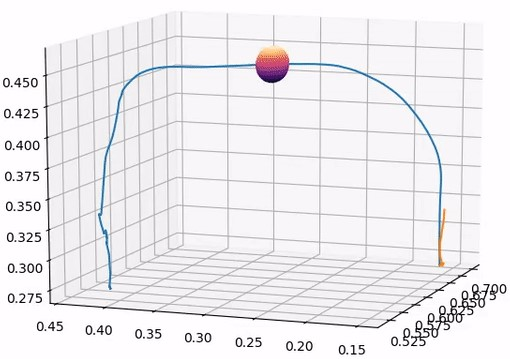
\includegraphics[width=\textwidth]{figures/online_obs/original_param/3D_ori_param-40.jpg}
        \caption{Frame 40 out of 281}
    \end{subfigure}
    \begin{subfigure}[b]{0.32\textwidth}
        \centering
        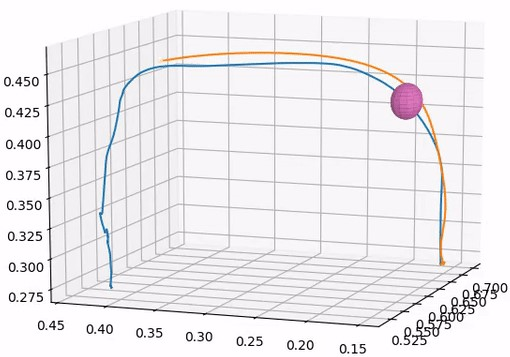
\includegraphics[width=\textwidth]{figures/online_obs/original_param/3D_ori_param-70.jpg}
        \caption{Frame 70 out of 281}
    \end{subfigure}
    \hfill
    \begin{subfigure}[b]{0.32\textwidth}
        \centering
        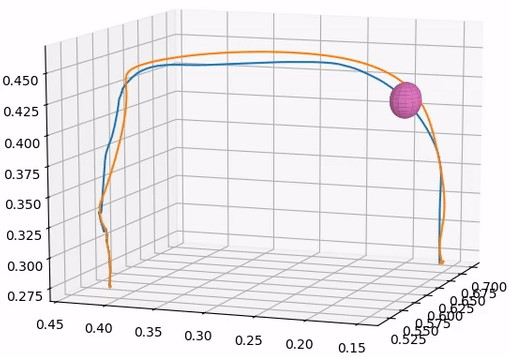
\includegraphics[width=\textwidth]{figures/online_obs/original_param/3D_ori_param-281.jpg}
        \caption{Frame 281 out of 281}
    \end{subfigure}
    \caption{Three steps of online obstacle avoidance using same tuning variable values as in \autoref{subsubsec:eval:pot:coupled:term}. Sphere's radius is $r=0.015[m]$, sphere's start point and end point is $start_{xyz}=[0.53, 0.39, 0.45]$ and $end_{xyz}=[0.65, 0.17, 0.41]$. Sphere follows the demonstrated path and stops moving when purple.}
    \label{fig:dmp:online:not:tuned}
\end{figure}

\autoref{fig:dmp:online:not:tuned} shows that the obstacle is not avoided thus the decouple terms are adjusted. The tuning variable values are modified to $\gamma_{1} = 3\cdot10^6$ and $\gamma_{3} = 2\cdot10^4$ in order to avoid the obstacle. The following tuning variable values can be seen in \autoref{fig:dmp:online:tuned} and visualized on Github\footnote{\url{https://github.com/Masle16/obstacle_avoidance_with_dmps/tree/dmp_online_obs_avoid/DMP}}

% \begin{figure}[H]
%  \centering
%  \animategraphics[loop,controls,width=\textwidth]{10}{figures/online_obs/tuned_param/mov_obs_param_tune-}{0}{69}
%  \caption{Animation of online obstacle avoidance using tuning variable values: $\gamma_1 = 3\cdot10^6$,  $\gamma_2=0$, $\gamma_3=2\cdot10^4$, $\beta_0 = \frac{20}{\pi}$, $k=15$ in order to avoid the obstacle}
%  \label{fig:dmp:online:tuned}
% \end{figure}

\begin{figure}[H]
    \centering
    \begin{subfigure}[b]{0.32\textwidth}
        \centering
        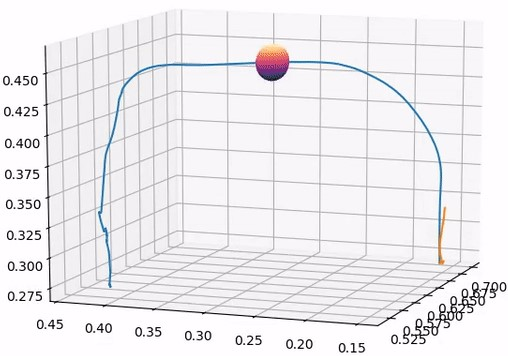
\includegraphics[width=\textwidth]{figures/online_obs/tuned_param/3D_tuned-40.jpg}
        \caption{Frame 40 out of 281}
    \end{subfigure}
    \begin{subfigure}[b]{0.32\textwidth}
        \centering
        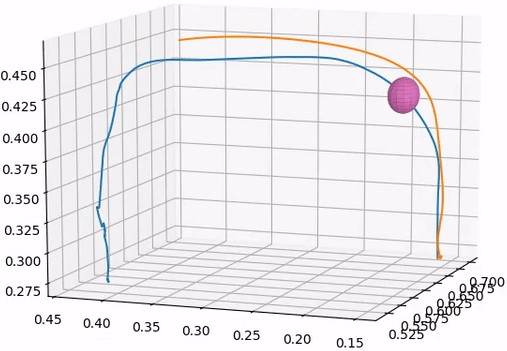
\includegraphics[width=\textwidth]{figures/online_obs/tuned_param/3D_tuned-70.jpg}
        \caption{Frame 70 out of 281}
    \end{subfigure}
    \hfill
    \begin{subfigure}[b]{0.32\textwidth}
        \centering
        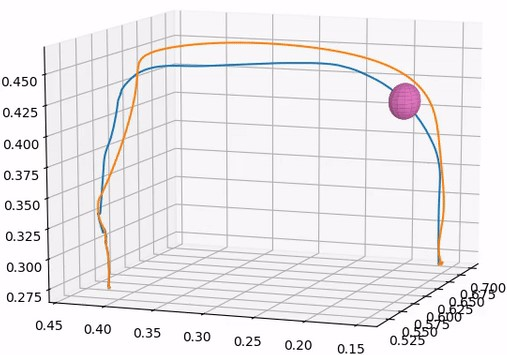
\includegraphics[width=\textwidth]{figures/online_obs/tuned_param/3D_tuned-281.jpg}
        \caption{Frame 281 out of 281}
    \end{subfigure}
    \caption{Three steps of online obstacle avoidance using tuning variable values: $\gamma_1 = 3\cdot10^6$,  $\gamma_2=0$, $\gamma_3=2\cdot10^4$, $\beta_0 = \frac{20}{\pi}$, $k=15$ in order to avoid the obstacle. Sphere's radius is $r=0.015[m]$, sphere's start point and end point is $start_{xyz}=[0.53, 0.39, 0.45]$ and $end_{xyz}=[0.65, 0.17, 0.41]$. Sphere follows the demonstrated path and stops moving when purple.}
    \label{fig:dmp:online:tuned}
\end{figure}

\subsection{Attraction Field Towards Demonstration \\ \normalfont\normalsize\texttt{Emil Vincent Ancker}}
To pull the end-effector back towards the demonstrated path after an obstacle has been encountered an attractional potential field is added to the demonstration. The potential field is defined to be a relationship between the positional error $\boldsymbol{x}_{demo} - \boldsymbol{x}$ and the euclidean distance to the obstacle $||(\boldsymbol{o} - \boldsymbol{x})||$.

\begin{equation} \label{eq:link:pot}
    U(\boldsymbol{x}) = \begin{cases}
      \gamma_T (\boldsymbol{x}_{demo} - \boldsymbol{x})e^{||(\boldsymbol{o} - \boldsymbol{x})||}, & ||(\boldsymbol{o} - \boldsymbol{x})|| > d_T \\
      0, & \text{otherwise}
    \end{cases}
\end{equation}
Where $\gamma_T$ is a constant defined the strength of the potential field and $d_T$ is a radius of non-influence meaning that within a certain distance of the obstacle the attraction towards the demonstrated trajectory should be ignored.

\subsubsection{Evaluation of Attraction Field \\ \normalfont\normalsize\texttt{Mikkel Larsen}}
The same path for both the DMP and the moving obstacle is used when evaluating the DMP with attraction field as in \autoref{fig:dmp:online:tuned}. Additionally the same tuning variables are kept as in \autoref{fig:dmp:online:tuned}. The threshold for when to activate the attractor field is set to $d_{T}=0.05$ and the potential attractor field strength is set to $\gamma_T = 2.5\cdot10^{3}$. This yields the following result shown in \autoref{fig:dmp:attractor:tuned}

\begin{figure}[H]
    \centering
    \begin{subfigure}[b]{0.32\textwidth}
        \centering
        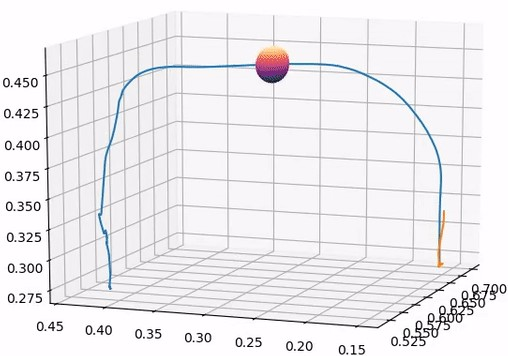
\includegraphics[width=\textwidth]{figures/online_obs/attractor/3D_tuned_w_attractor-40.jpg}
         \caption{Frame 40 out of 281}
    \end{subfigure}
    \begin{subfigure}[b]{0.32\textwidth}
        \centering
        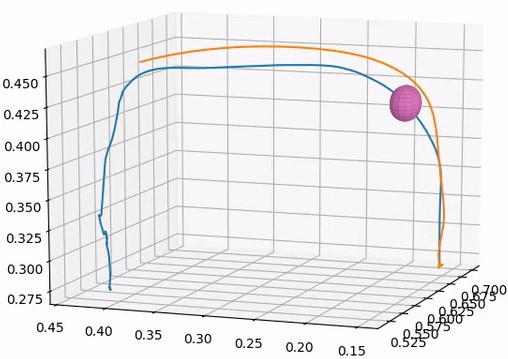
\includegraphics[width=\textwidth]{figures/online_obs/attractor/3D_tuned_w_attractor-70.jpg}
         \caption{Frame 70 out of 281}
    \end{subfigure}
    \hfill
    \begin{subfigure}[b]{0.32\textwidth}
        \centering
        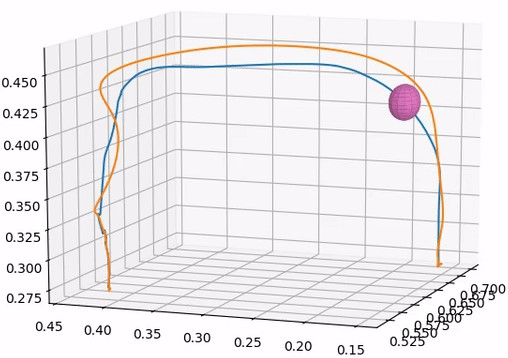
\includegraphics[width=\textwidth]{figures/online_obs/attractor/3D_tuned_w_attractor-281.jpg}
         \caption{Frame 281 out of 281}
    \end{subfigure}
    \caption{Three steps of online obstacle avoidance with attractor field using the same tuning variable values as in \autoref{fig:dmp:online:tuned}. The attractor field parameters were set to $d_{T}=0.05$ and $\gamma_T = 2.5\cdot10^{3}$. Sphere's radius is $r=0.015[m]$, sphere's start point and end point is $start_{xyz}=[0.53, 0.39, 0.45]$ and $end_{xyz}=[0.65, 0.17, 0.41]$. Sphere follows the demonstrated path and stops moving when purple.}
    \label{fig:dmp:attractor:tuned}
\end{figure}

To quantify the performance of the attractor DMP method versus without the attractor field the euclidean distance between the demonstrated position and DMP position is found. This is illustrated in \autoref{fig:tuned:vs:attractor} for the tuned online obstacle avoidance DMP versus the attraction field DMP. 

\begin{figure}[H]
    \centering
         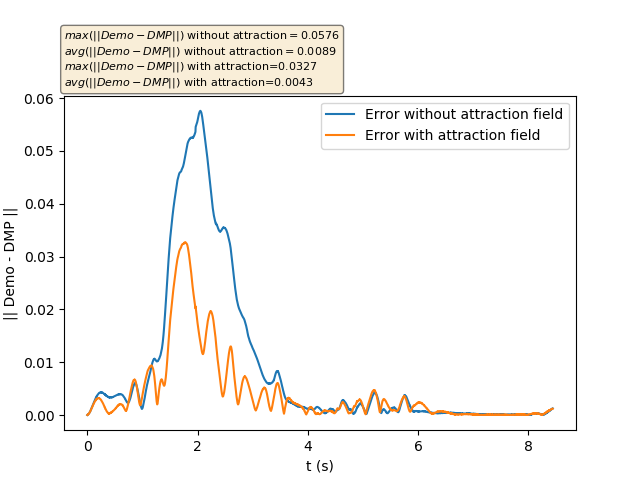
\includegraphics[width=0.6\textwidth]{figures/eval_trajectories/online-dmp_v_attractor-dmp.png}
     \caption{Euclidean distance between the demonstrated path and the DMP generated paths for DMP online obstacle avoidance and DMP with Attraction Field.}
     \label{fig:tuned:vs:attractor}
\end{figure}

From \autoref{fig:tuned:vs:attractor} it is seen that using an attractor field while doing online obstacle avoidance makes the DMP generated path follows the demostrated path more accurate compared to not using an attractor field. However, it can also be seen that using an attractor field makes oscillations in the euclidean distance when trying to avoid the obstacle around the $2$ seconds mark. The DMP with attractor term has $43.2 \%$ smaller maximum euclidean distance and $51.7 \%$ smaller average euclidean distance compared to DMP with coupling terms


% \subsection{Fitting Potential Fields to Demonstration  \\ \normalfont\normalsize\texttt{Emil Vincent Ancker}}
% \todo{write and test}
% \begin{equation} \label{eq:repulsive:fit}
%     \tau^2 \ddot{\boldsymbol{x}} = \alpha_z ( \beta_z (g-\boldsymbol{x}) - \tau \dot{\boldsymbol{x}}) + f + C_t
% \end{equation}
% Leads to,
% \begin{equation} \label{eq:repulsive:iso}
%     \tau^2 \ddot{\boldsymbol{x}} - \alpha_z ( \beta_z (g-\boldsymbol{x}) - \tau \dot{\boldsymbol{x}}) - f =  C_t
% \end{equation}
% Where,
% \begin{equation}
% C_t = A_1 \gamma_1 + A_2 \gamma_2 + A_3 \gamma_3    
% \end{equation}
% Each element is 3-dimensional.
% Can be put on matrix form,
% \begin{equation}
%     \underset{(K \times 3)}{\boldsymbol{A}} = \begin{bmatrix} A_1(0) & A_2(0) & A_3(0) \\ A_1(1) & A_2(1) & A_3(1) \\ A_1(K) & A_2(K) & A_3(K) \end{bmatrix}, \quad \Gamma = \begin{bmatrix} \gamma_1 \\ \gamma_2 \\ \gamma_3 \end{bmatrix} 
% \end{equation}
% The left hand side in \autoref{eq:repulsive:iso} is now denoted $C_{target}$ and is put on matrix form,
% \begin{equation}
%     \underset{(K\times 1)}{\boldsymbol{C}} = \begin{bmatrix} \tau^2 \ddot{\boldsymbol{x}}_0 - \alpha_z ( \beta_z (g-\boldsymbol{x}_0) - \tau \dot{\boldsymbol{x}}_0) - f_0 \\ \tau^2 \ddot{\boldsymbol{x}}_1 - \alpha_z ( \beta_z (g-\boldsymbol{x}_1) - \tau \dot{\boldsymbol{x}}_1) - f_1 \\ \vdots \\ \tau^2 \ddot{\boldsymbol{x}}_K - \alpha_z ( \beta_z (g-\boldsymbol{x}_K) - \tau \dot{\boldsymbol{x}}_K) - f_K \end{bmatrix}
% \end{equation}
% This can be solved by,
% \begin{equation}
%     \boldsymbol{A}\Gamma = \boldsymbol{C}
% \end{equation}

\end{document}